\chapter{Experiments and Results}
%\addcontentsline{toc}{chapter}{Experiments and results}

\section{Experimental Setup}
	Thanks to the configurability of the programme we were able to run the majority of experiments in a batch processing mode. That is, we wrote a script in bash that allowed running multiple tests in series without any maintenance. In a single series of tests any parameters could be modified or any data processing algorithm could be exchanged. All experiments were run on a notebook with Intel Core i7 quad core 2.2 GHz CPU, 8 GB of RAM and a nVidia M540 GPU.

\section{Experiments}	
	As already stated, a BoW pipeline consists of:
	\begin{inparaenum}[\upshape(1\upshape)]
	\item keypoint detection
	\item feature extraction 
	\item vector quantization and
	\item classification.
	\end{inparaenum}
	The number of possible combinations grows combinatorial with the amount of candidates for each part. We have to bear in mind that each algorithm contains a set of parameters that have to be adjusted for optimal performance. It would require a great deal of time and computational power to conduct exhaustive evaluation. Even if we consider only a single library --- PCL, we would have far too many options with 12 keypoint detectors and more than 20 feature descriptors. A literature review can help perform an early selection of algorithms.	
	
	\subsection{Detectors and descriptors}
	Keypoint detection algorithms have been compared with respect to repeatability, invariance in \cite{pcl_keypoint_comparision} and in terms of object retrieval and recognition in \cite{3d_keypoint_eval}. 3D-SIFT and ISS achieve the highest robustness for invariance, while the latter appears to be the best choice for object retrieval. Dense detector (or uniform sampling) achieved the best performance in 2D image classification \cite{tsai2012bag}. Therefore, this paper compares SIFT, ISS and Uniform Sampling keypoint detection techniques. 
	
	PCL descriptors have been evaluated in terms of object retrieval performance in \cite{pcl_features}. PFHRGB and SHOTCOLOR delivered the best performance, while their simpler counterparts (PFH, FPFH, SHOT) were only a little worse. USC, which is a global descriptor and thus not suitable for the Bag of Words approach, achieved very similar accuracy. We focus on the family of PFH algorithms.
	
	\begin{table}[!ht]
	\centering	
	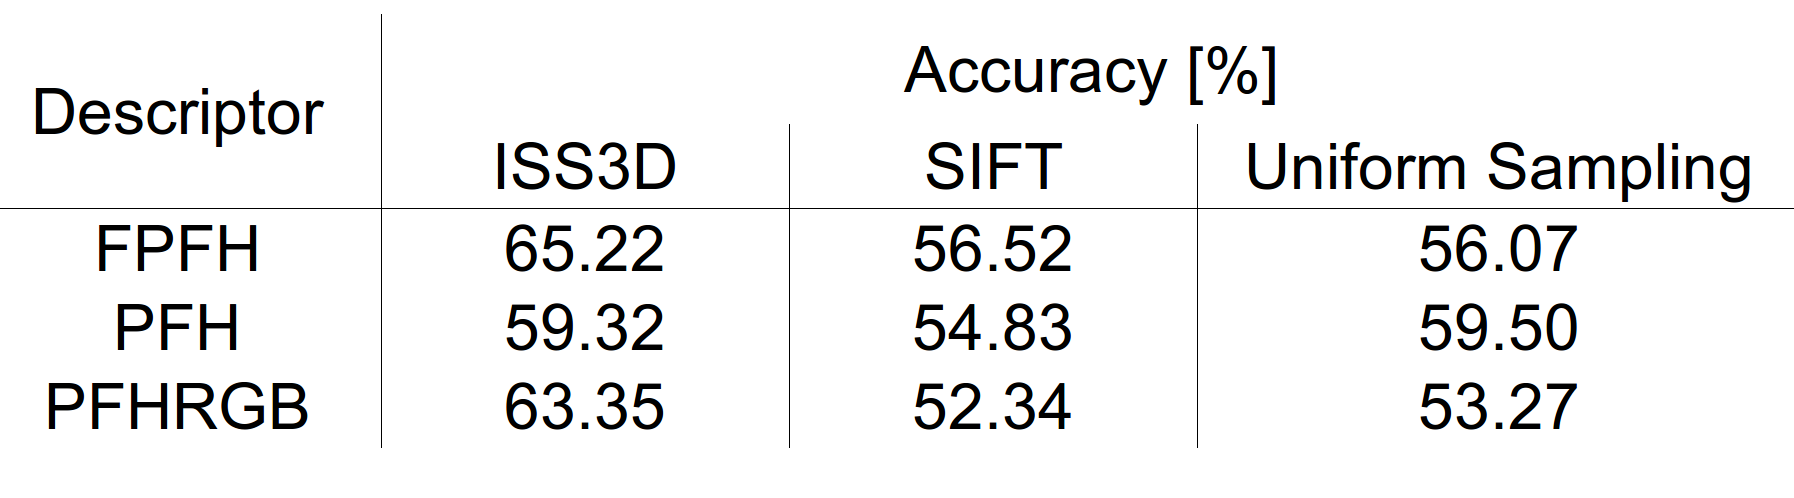
\includegraphics[width=.55\textwidth]{figs/desc_b3do}
	\caption{Highest accuracy obtained with FPFH, PFH and PFHRGB descriptors on the B3DO dataset}
	\label{tab:desc_b3do}
	\end{table}
	
	The best results achieved are shown in the figure \ref{tab:desc_b3do}. They were scored on the B3DO dataset. As for the detection algorithms, the ISS provided consistently the highest accuracy. The SIFT and Uniform Sampling provide very similar accuracy, but the latter is significantly faster. SIFT is in fact slowest of the three. As for the descriptors, the FPFH delivered the best performance even though it is an approximate and theoretically the least precise algorithm. It is also the fastest of the three. It appears that the combination of ISS and FPFH is not only surprisingly good in terms of accuracy, but it is also the fastest. These two algorithms allow near real time point-cloud processing and classification. PFHRGB and SIFT are several times slower.
		
	\subsection{Codebook}
	KMeans is used in almost every implementation of the Bag of Words image processing pipeline \cite{tsai2012bag, toldo2009bag}. Csurka \emph{et al} showed that the number of visual words has a significant impact on the final results \cite{csurka2004visual}. We run a number of tests to discover an optimal codebook size for our setting.
	
	\begin{figure}[!ht]
	\centering	
	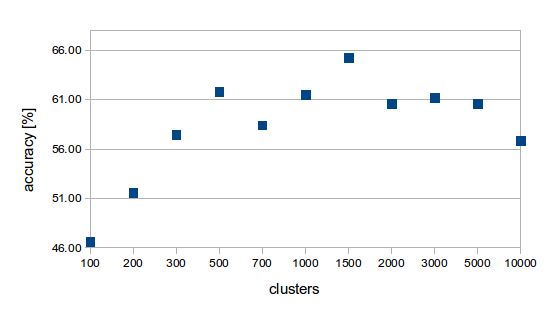
\includegraphics[width=.75\textwidth]{figs/clustering_centroids_b3do}
	\caption{Influence of dictionary size on the overall accuracy. B3DO dataset with ISS keypoint detector and FPFH feature descriptor}
	\label{fig:cluster_b3do}
	\end{figure}
	
	The results from the figure \ref{fig:cluster_b3do} partially confirm Csurka's findings. The performance raises with the increasing number of centroids up to the point of 1500 centroids and 65.22\%. The discrepancies might be caused by the following factors: (1) ISS detector finds too many or irrelevant points, thus introducing noise or (2) The FPFH descriptor has too few dimensions (33) to be divided into more than 1500 regions in a meaningful way. 

	
	\subsection{B3DO}
	The majority of the point clouds in the B3DO dataset contain several different objects. We have extracted every individual object from the clouds and divided them into 78 separate categories. Unfortunately, they were badly balanced \emph{i.e.} the number of objects in a category varies from 1 (tape) to 299 (table). We have picked 8 categories at random with a restriction that there should be at least 50 object instances in a category. Then, the objects were split into two sets (training and testing) with a proportion of 1:1. As the names suggest, they are used for estimation and evaluation respectively.
	
	The highest accuracy achieved for this dataset is 64\%. Table \ref{tab:b3do_conf_matrix} contains a confusion matrix, number of examples per category and accuracy. The confusion matrix depicts classification errors. Let m\subscript{i, j} be an element of the confusion matrix at the i\superscript{th} row and j\superscript{th} column. It shows how many elements from the i\superscript{th} category was assigned to the j\superscript{th} category. A high value of m\subscript{i, j} such that $i \neq j$ indicates that the classifier cannot distinguish between those two classes.
	
	\begin{table}[!ht]
	\centering
	\caption{Results on the B3DO dataset with ISS keypoint detector, FPFH features and a dictionary of 1500 words. \textbf{Overall accuracy is 65.22\%}}
	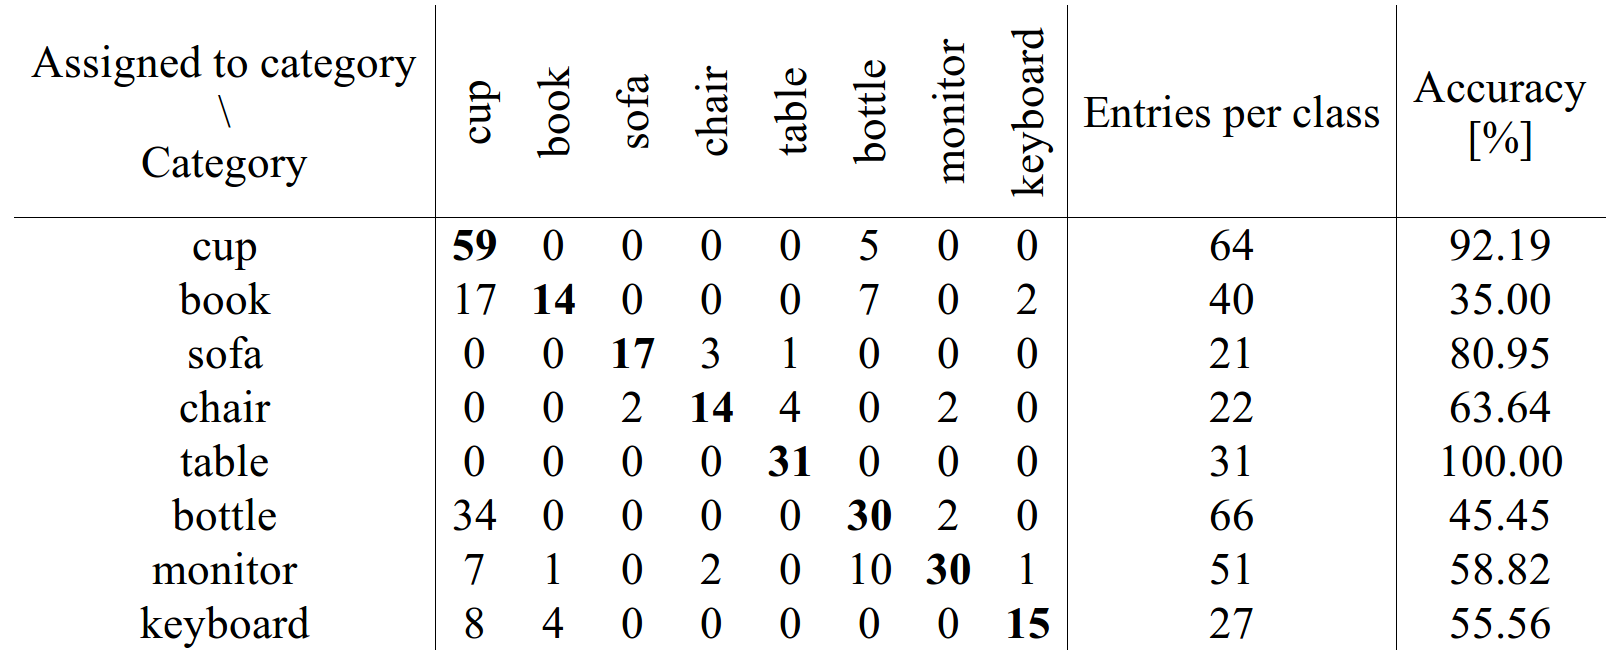
\includegraphics[width=0.9\textwidth]{figs/b3do_conf_matrix}	
	\label{tab:b3do_conf_matrix}
	\end{table}
	
	\begin{figure}[!ht]
	\centering	
	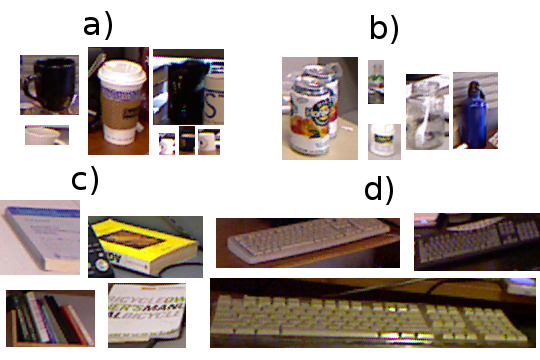
\includegraphics[width=.75\textwidth]{figs/b3do_objects}
	\caption{B3DO objects. Images are in their original sizes. a) cups b) bottles c) books d) keyboards}
	\label{fig:b3do_objects}
	\end{figure}
	
	More than half of the bottles were assigned to the cup category and keyboards were often mistook for books. These two error types are easily explained by a high degree of similarity of objects (bottles and cups are usually round and tall, books and keyboards are flat and rectangular) Surprisingly, however, objects from half of the categories were frequently marked as cups. Some of these misclassification errors might be caused by very poor quality of images. Many of them are occluded poorly lit low resolution images.	
	
	\subsection{Tokyo}
	\begin{table}[!ht]
	\centering
	\caption{Tokyo confusion matrix with ISS keypoint detector, PFH features and a dictionary of 3000 words}
	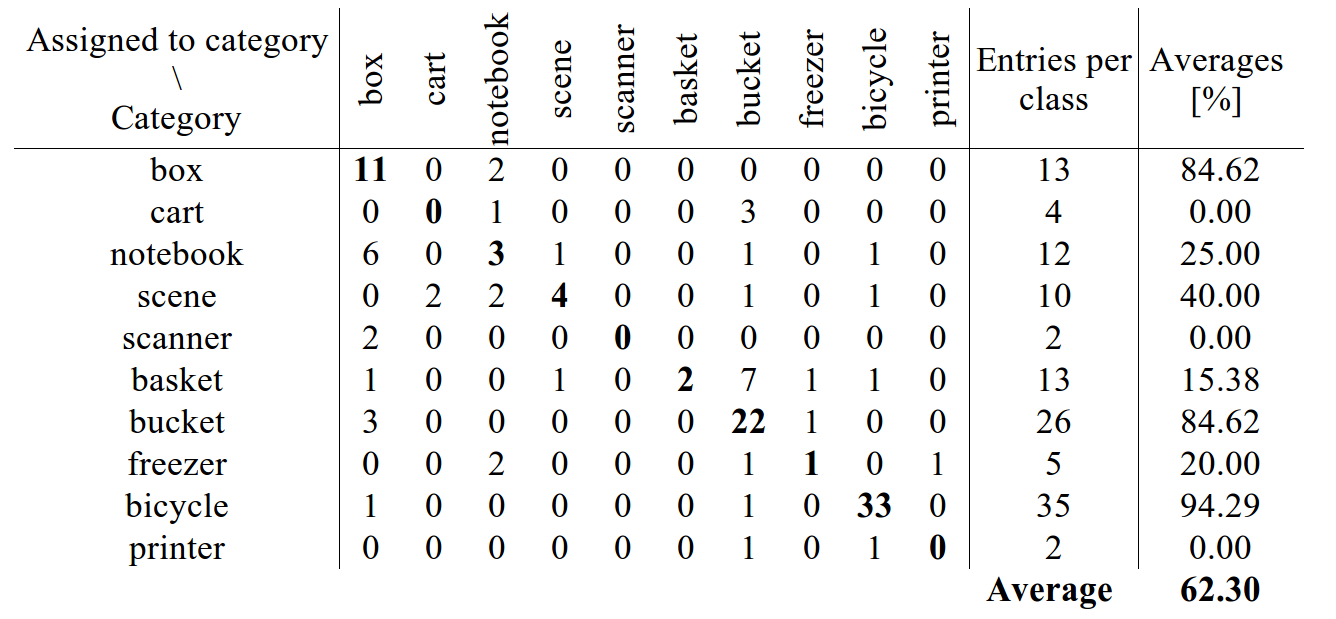
\includegraphics[width=0.9\textwidth]{figs/tokyo_conf_matrix}	
	\label{tab:tokyo_conf_matrix}
	\end{table}
	
	Every of the 343 images from Tokyo dataset was used. Data was split into test and train set in proportions 1:2 in order to provide more training examples due to low number of objects in some classes.
	
	Even tough the overall accuracy achieved on Tokyo dataset is similar in value to that of the B3DO, the structure of the result is very different. It is clearly visible that there is a strong correlation between a per class accuracy and the number of entries in this class. The highest performance in the bicycle category is coupled with the largest number of entries. On the other end of the scale there are cart and printer categories with only 2 and 4 entries respectively. On top of that there are differences between some classes are marginal. The majority of carts and baskets were put into the bucket category. It does not surprise, for they are simply akin as can be seen in figure \ref{fig:tokyo} on the page \pageref{fig:tokyo}.
	
\section{Conclusion}

	In this paper we have tackled the issue of three dimensional point cloud classification with a bag of words-based approach. The main focus was put on the design and efficient implementation of the pipeline in a way that allows easy addition of algorithms and switching them at run-time. What is more, we have gone to great lengths in order to find scientific databases that are suitable for the task of point cloud classification. We believe that the presence of such databases is fundamental, for it allows meaningful comparison with other researchers. We have experienced the following problems: Firstly, point cloud processing is computationally expensive and inefficient. Due to the lack of structure in point clouds (\textit{i.e.} no predefined relationship between points) additional calculations have to be performed (\textit{e.g.} finding nearest neighbours requires distance comparison for all points in a cloud, whereas for a 2D image one instantly knows where adjacent pixels lie). Secondly, there are virtually no databases that would allow extensive training of the bag of words-based pipeline. Machine learning algorithms have ravenous appetite for labelled data. As the newest findings in the state-of-the-art 2D object classification suggest, an order of tens of thousands of samples is a prerequisite for any satisfactory results We had to make do with as few as 330 objects in our training set. Moreover, there is very little interest in the scientific community for this particular task. The majority of research is conducted on retrieval of CAD-like objects from mesh databases. Last, but not least, there is no 3D detection or description algorithm designed solely for the purpose of bag of words object classification.
	
	In conclusion I would not recommend any bag-of-words based approach classification of real point clouds registered with a low quality camera such as Microsoft Kinect. Being computationally expensive and rather inefficient, it delivers inferior performance in terms of accuracy and speed when compared to 2D RGB image based algorithms. To makes matters worse, generalisation of 2D algorithms to the 3D domain can be very involved, causing the cutting-edge inventions of the 2D image processing scientists unavailable for the purpose of 3D point cloud processing.